\Subsection{Система множеств}
Полезные оьозначения: $A \sqcup B$ - объединение $A$ и $B$, такие что $A \cap B = \emptyset$

\begin{definition}
    Набор мн-в дизъюнктный, если мн-ва попарно не пересекаются: $\bigsqcup_{\alpha \in I}A_{\alpha}$
\end{definition}

\begin{definition}
    $E$ -- мн-во; если $E = \bigsqcup_{\alpha \in I} E_{\alpha}$ -- разбиение мн-ва $E$.
\end{definition}

Напоминание:
$$X \setminus \bigcup_{\alpha \in I} A_{\alpha} = \bigcap X \setminus A_{\alpha}$$
$$X \setminus \bigcap_{\alpha \in I} A_{\alpha} = \bigcup X \setminus A_{\alpha}$$


\begin{definition}
    $\mathcal{А}$ -- система подмн-в $X$: $A \subset 2^{X}$

    \begin{enumerate}
        \item ($\delta_0$) если $\forall A, B \in \mathcal{A} \implies A \cap B \in \mathcal{A}$
        \item ($\sigma_0$) если $\forall A, B \in \mathcal{A} \implies A \cup B \in \mathcal{A}$
        \item {
            $(\delta)$ если $A_n \in \mathcal{A}, \ \forall n \implies \bigcap_{n=1}^{\infty} A_n \in \mathcal{A}$
        }
        \item {
            $(\sigma)$ если $A_n \in \mathcal{A}, \ \forall n \implies \bigcup_{n=1}^{\infty} A_n \in \mathcal{A}$
        }
    \end{enumerate}
\end{definition}

\begin{definition}
    $\mathcal{A}$ -- симметрическая система мн-в, если $\forall A \in \mathcal{A} \implies X \setminus A \in \mathcal{A}$.
\end{definition}

\begin{statement}
    Если $\mathcal{A}$ -- симм., то $(\delta_{0}) \Leftrightarrow (\sigma_{0})$ и $(\delta) \Leftrightarrow (\sigma)$.
\end{statement}

\begin{proof}
    $A_{\alpha \in I}\mathcal{A} \Leftrightarrow X \setminus A_{\alpha} \in \mathcal{A} \implies \bigcup_{\alpha \in I}A_{\alpha} = \bigcap_{\alpha \in I} X \setminus A_{\alpha} \in \mathcal{A}$
\end{proof}

\begin{definition}
    $\mathcal{A}$ -- алгебра мн-в, если $\mathcal{A}$ -- симметр., $\emptyset \in \mathcal{A}$ и $\forall A, \ B \in \mathcal{A}: \ A \cup B \in \mathcal{A}$ (по утв. 1.1 $(\delta_0) \Leftrightarrow (\sigma_0)$; смотри \href{https://ru.wikipedia.org/wiki/%D0%90%D0%BB%D0%B3%D0%B5%D0%B1%D1%80%D0%B0_%D0%BC%D0%BD%D0%BE%D0%B6%D0%B5%D1%81%D1%82%D0%B2#%D0%9E%D0%BF%D1%80%D0%B5%D0%B4%D0%B5%D0%BB%D0%B5%D0%BD%D0%B8%D0%B5}{опр. алгебры}).
\end{definition}

\begin{properties}
    алгебры мн-в: 

    \begin{enumerate}
        \item {
            $\emptyset, X \in \mathcal{A}$
        }
        \item Если $A_1, \dots, A_n \in \mathcal{A}$, то $\bigcup_{k = 1}^n A_k \in \mathcal{A} \land \bigcap_{k = 1}^n A_k \in \mathcal{A}$
        \item Если $A, B \in \mathcal{A}$, то $A \cap (X \setminus B) = A \setminus B \in \mathcal{A}$
    \end{enumerate}
\end{properties}

\begin{definition}
    $\mathcal{A}$ - \sigma-алгебра мн-в, если $\mathcal{A}$ -- симм., $\emptyset \in \mathcal{A}$ и свойство (\sigma) выполнено (т.е. есть замкнутость по объединению любого числа множетсв; в силу симметричности по утв. 1.1 получаем $(\sigma) \Leftrightarrow (\delta)$).
\end{definition}

\begin{remark}
    \sigma-алгебра $\implies$ алгебра.
\end{remark}

\begin{example}
    \begin{enumerate}
        \item $2^X$ - \sigma-алгебра.
        
        \item $X = \mathbb{R}^2$, $\mathcal{A}$ - всевозможные \href{https://ru.wikipedia.org/wiki/%D0%9E%D0%B3%D1%80%D0%B0%D0%BD%D0%B8%D1%87%D0%B5%D0%BD%D0%BD%D0%BE%D1%81%D1%82%D1%8C}{огр. подмн-ва.} $\mathbb{R}^2$ и их дополнения. ($\mathcal{A}$ -- алгебра, но не \sigma-алгебра).
        
        \textbf{Rem}: огр. множество - в метрич. пр-ве это множетсво ограниченного диаметра ($d(x, \ y) := || x - y ||$), т.е. $sup\{ d(x, \ y) \ | x, \ y \in X \}$ - ограничен.

        \item $\mathcal{A}$ - алгебра (\sigma-алгебра) подмн-в $X$ и $Y \subset X$. $\mathcal{A}_{Y} := \{A \cap Y : A \in \mathcal{A}\}$ -- индуцированная алгебра (\sigma-алгебра).
        
        \item Пусть $\mathcal{A}_{\alpha}$ -- алгебры (\sigma-алгебры), тогда $\bigcap_{\alpha \in I}\mathcal{A}_{\alpha}$ -- алгебра (\sigma-алгебра).
        
        \item $A, B \subset X$ что есть в адгебра, содержащей $A, B$: \\ $\emptyset, X, A, B, A \cup B, A \cap B, A \setminus B, B \setminus A, X \setminus A, X \setminus B, X \setminus (A \cup B), X \setminus (A \cap B), A \vartriangle B, X \setminus (A \vartriangle B), X \setminus (A \setminus B), X \setminus (B \setminus A)$.
    \end{enumerate}
\end{example}

\begin{theorem}
    Пусть $\epsilon$ -- семейство подмн-в в $X$, тогда существует наименьшая по включению \sigma-алгебра (алгебра) $\mathcal{A}$, такая что $\epsilon \subset \mathcal{A}$.
\end{theorem}

\begin{proof}
    $\mathcal{A}_{\alpha}$ -- всевозможные \sigma-алгебры $\supset \epsilon$. Такие есть, так как $2^X$ подходит.

    $\mathcal{A} := \bigcap_{\alpha \in I} \mathcal{A}_{\alpha} \supset \epsilon$. Теперь проверим, что $\mathcal{A}$ -- наим. по вкл. $\mathcal{A} \subset A_{\alpha}$ $\forall \alpha \in I$.

    \begin{definition}
        \begin{enumerate}
            \item Такая \sigma-алгебра -- борелевская оболка $\epsilon$ -- $(\mathcal{B}(\epsilon))$.
            
            \item $X = \mathbb{R}^n$; такая \sigma-алгебра, натянутая на все открытые мн-ва -- борелевская \sigma-алгебра $(\mathcal{B}^n)$.
        \end{enumerate}
    \end{definition}

    \begin{remark}
        континуальное -- $\mathcal{B}^n \neq 2^{\mathbb{R}^n}$ -- больше.
    \end{remark}
\end{proof}

\begin{definition}
    $R$ -- кольцо, если $\forall A, B \in R \implies A \cup B, A \cap B, A \setminus B \in R$.
\end{definition}

\begin{remark}
    Кольцо + $(X \in R) \implies$ алгебра.
\end{remark}

\begin{definition}
    $P$ -- полукольцо, если 
    \begin{enumerate}
        \item $\emptyset \in P$
        \item $\forall A, B \in P \implies A \cap B \in P$
        \item $\forall A, B \in P \implies \exists Q_1, Q_2, \dots, Q_n \in P$, такие что $A \setminus B = \bigsqcup_{k = 1}^{n}Q_k$.
    \end{enumerate}
\end{definition}

\begin{example}
    $X = \mathbb{R}, P = \{(a, b] : a, b \in X\}$ -- полукольцо.

    \hbox{
        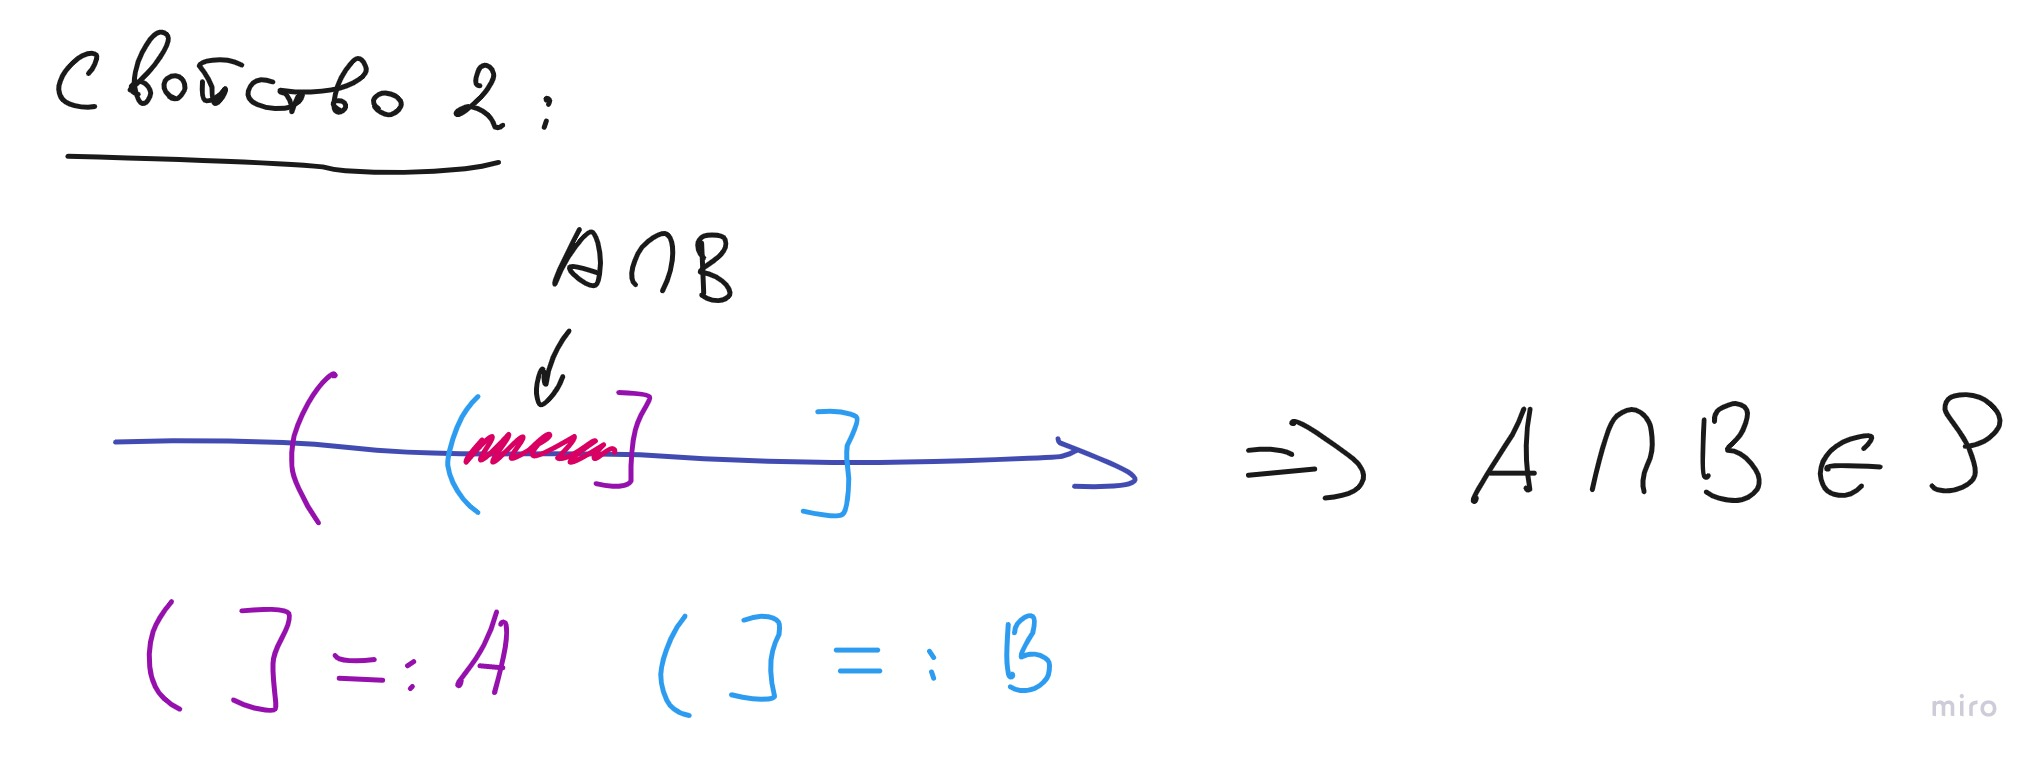
\includegraphics[scale=0.15]{./assets/01-measure-theory/semicircle-prop-2.jpg}
    }
    \hbox{
        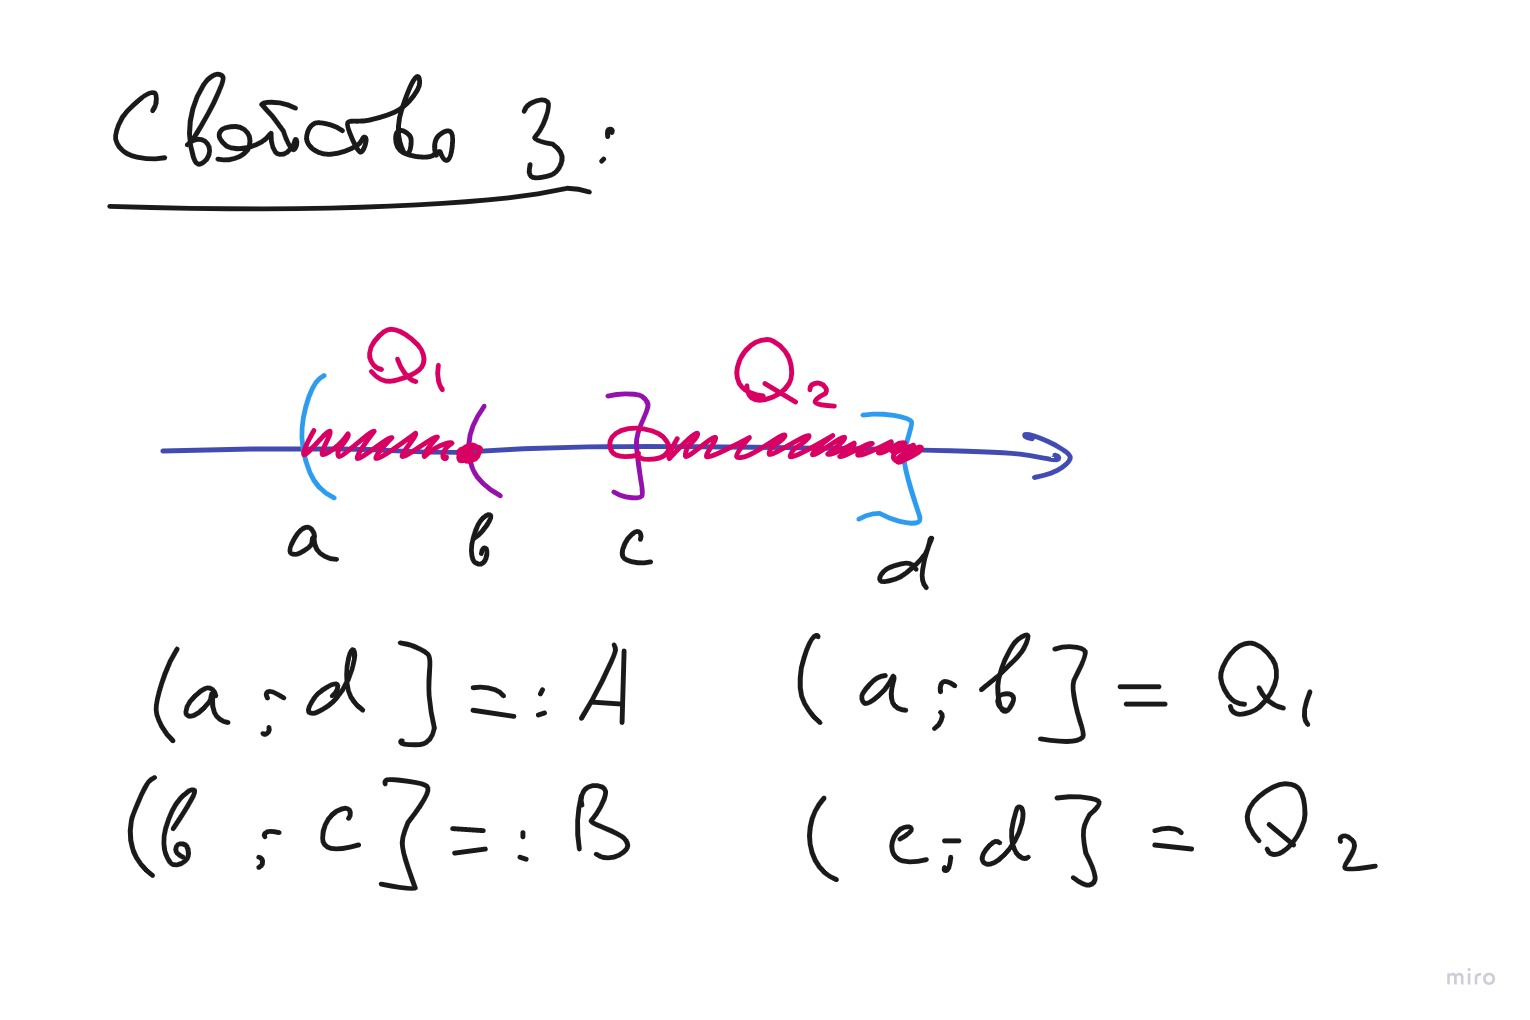
\includegraphics[scale=0.15]{./assets/01-measure-theory/semicircle-prop-3.jpg}
    }

\end{example}

\begin{lemma}
    $\bigcup_{n=1}^{N} A_n = \bigsqcup_{n=1}^{N}A_n \setminus \underbrace{\left(\bigcup_{k=1}^{n-1}A_k\right)}_{B_n}$.
\end{lemma}
\begin{proof}
    $\supset$: Дизъюнктивность $B_n \subset A_n $ и при $m > n$ $B_m \cap A_n = \emptyset \implies B_n \cap B_m = \emptyset$.
    
    $\subset$: Пусть $x \in \bigcup_{n=1}^{N} A_n$. Возьмем наим. $m$, такой что $x \in A_m \implies x \in B_m \implies x \in \bigsqcup_{n=1}^{N} B_n$.
\end{proof}

\begin{theorem}
    $P, P_1, P_2, \dots \i \mathcal{P}$. Тогда 

    \begin{enumerate}
        \item $P \setminus \bigcup_{k=1}^{n} P_k = \bigsqcup_{j=1}^m Q_j$, где $Q_j \in \mathcal{P}$ -- полукольцо.
        \item $\bigcup_{k=1}^{n} P_k = \bigsqcup_{k=1}^{n} \bigsqcup_{j=1}^{m_k} Q_{kj}$, где $Q_{kj} \in \mathcal{P}$ и $Q_{kj} \subset P_k$. 
    \end{enumerate}
\end{theorem}

\begin{proof}
    \begin{enumerate}
        \item индукция по n. База -- опр. полукольца. Переход ($n \rightarrow n+1$): $P \setminus \bigcup_{k=1}^{n+1}P_k = \left(P \setminus \bigcup_{k=1}^nP_k\right) \setminus P_{k+1} = \bigsqcup_{j=1}^{m} \left(\underbrace{Q_j \setminus P_{n+1}}_{\bigsqcup_{i=1}^{l_j}Q_{ji}}\right)$
        \item $\bigcup_{k=1}^{n} P_k = \bigsqcup_{k=1}^{n} \left(\underbrace{P_k \setminus \bigcup_{j=1}^{k-1} P_j}_{\bigsqcup_{j=1}^{m_k} Q_{kj}}\right)$
    \end{enumerate}
\end{proof}

\begin{remark}
    В (2) можно писать $n = \infty$.
\end{remark}

\begin{definition}
    $\mathcal{P}$ -- полукольцо подмн-ва $X$.

    $\mathcal{Q}$ -- полукольцо подмн-ва $Y$.

    $\mathcal{P} \times \mathcal{Q} := \{P \times Q : P \in \mathcal{P}, Q \in \mathcal{Q}\}$ -- декартово произведение полуколец.
\end{definition}

\begin{theorem}
    Декартово произведение полуколец -- полукольцо.
\end{theorem}
\begin{proof}
    
    $$(P \times Q) \cap (P' \times Q') = (P \cap P') \times (Q \cap Q')$$

    $$(P \times Q) \setminus (P' \times Q') = (P \setminus P') \times Q \sqcup (P \cap P') \times (Q \setminus Q')$$
\end{proof}

\begin{remark}
    Остальные структуры не сохр. при декартовом произведении: $2^X \times 2^Y$ -- полукольцо.
\end{remark}

\begin{definition}
    Замкнутый параллелепипед $a, b \in \mathbb{R}^m$.

    $[a, b] = [a_1, b_1] \times [a_2, b_2] \times \dots \times [a_m, b_m]$

    Открытый параллелепипед:

    $(a, b) = (a_1, b_1) \times (a_2, b_2) \times \dots \times (a_m, b_m)$

    Ячейка:
    
    $(a, b] = (a_1, b_1] \times (a_2, b_2] \times \dots \times (a_m, b_m]$
\end{definition}

\begin{theorem}
    Непустая ячейка -- перечисление убыв. посл. открытых паралл. / объединение возраст. послед. замкн.
\end{theorem}

\begin{proof}

    $P_n := (a_1, b_1 + \frac{1}{n}) \times \dots \times (a_m, b_m + \frac{1}{n})$

    $P_n \supset P_{n+1}$ и $\bigcap_{n=1}^{\infty}P_n = (a, b]$

    $Q_n := [a_1 + \frac{1}{n}, b_1] \times \dots \times [a_m + \frac{1}{n}, b_m]$

    $Q_n \subset Q_{n+1}$ и $\bigcup_{n=1}^{\infty}Q_n = (a, b]$ 

    \hbox{
        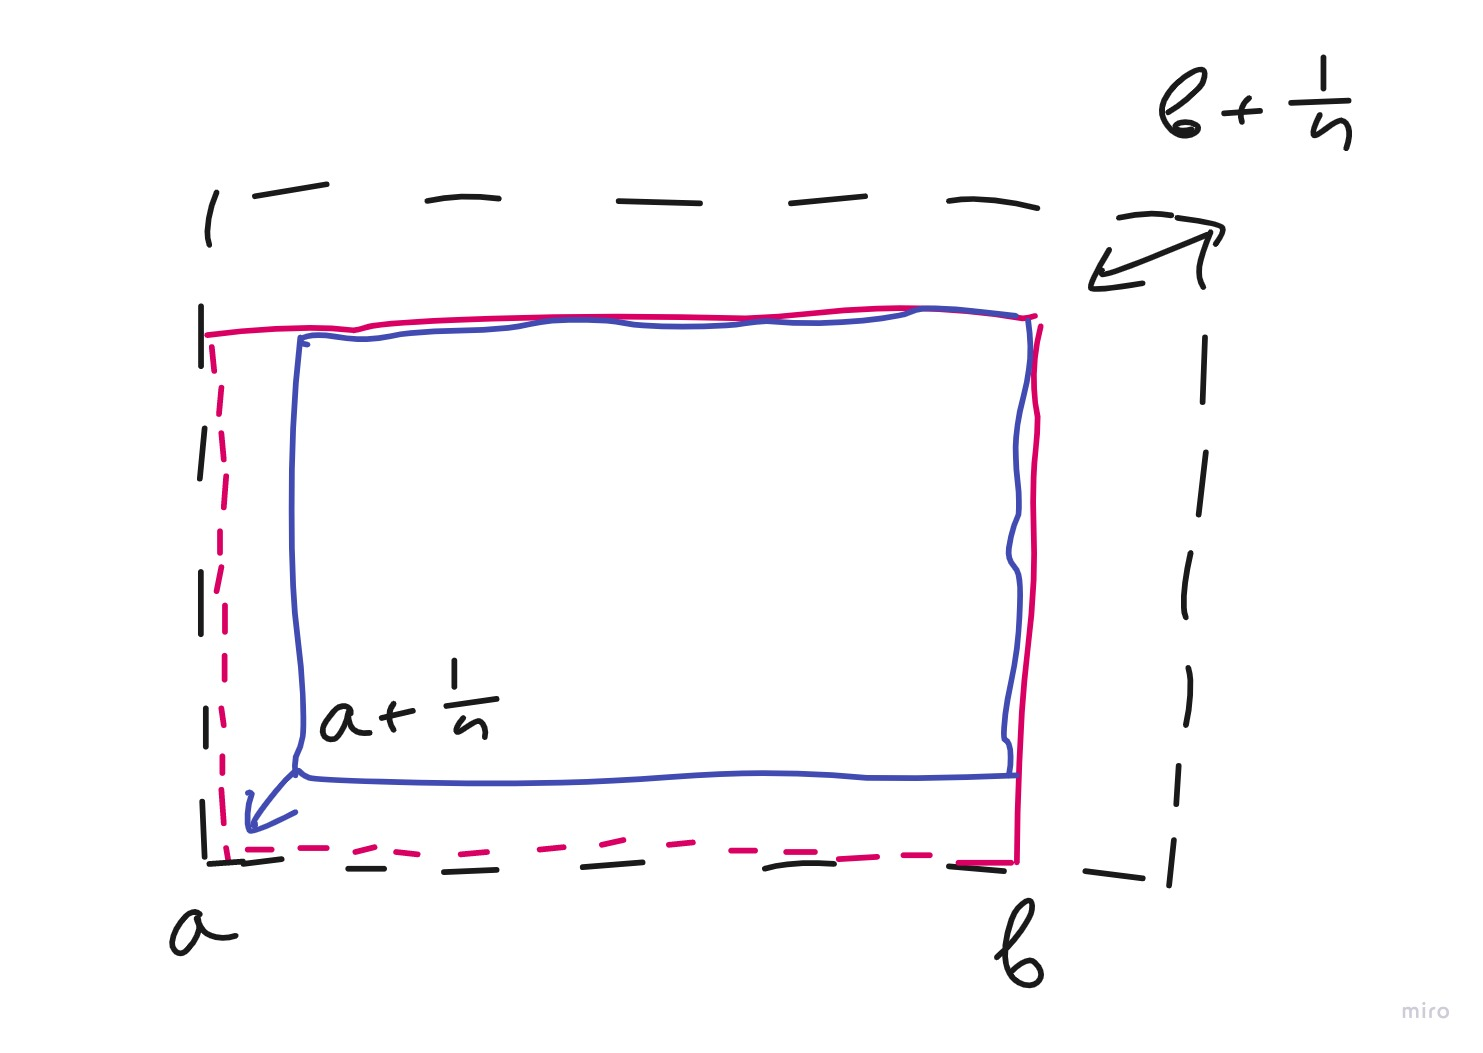
\includegraphics[scale=0.15]{./assets/01-measure-theory/rects-1.jpg}
    }

\end{proof}

\textbf{Обозначения}: $\mathcal{P}^m$ -- сем-во ячеек из $\mathbb{R}^m$.

$\mathcal{P}_{Q}^{m}$ -- сем-во ячеек из $\mathbb{R}^m$ с рациональными координатами вершин.

\begin{theorem}
    $\mathcal{P}^m, \mathcal{P}^m_Q$ -- полукольца.
\end{theorem}
\begin{proof}
    $\mathcal{P}^m = \mathcal{P}^{m-1} \times \mathcal{P}^1$

    $\mathcal{P}_Q^m = \mathcal{P}_Q^{m-1} \times \mathcal{P}_Q^1$
\end{proof}

\begin{theorem}
    $G \neq \emptyset$ -- открытое множество в $\mathbb{R}^m$. Тогда его можно представить как не более чем счетное дизъюнктивное объелинение ячеек, замыкание каждой из которых содержится в $G$ (можно считать, что ячейки с рациональными координатными вершинами).
\end{theorem}
\begin{proof}

    $R_x$ -- ячейка, $\underbrace{Cl  (R_x)}_{\text{замыкание ячейки}} \subset G$, $x \in R_x$, получаем, что $G = \bigcup_{x \in G} R_x$.

    \hbox{
        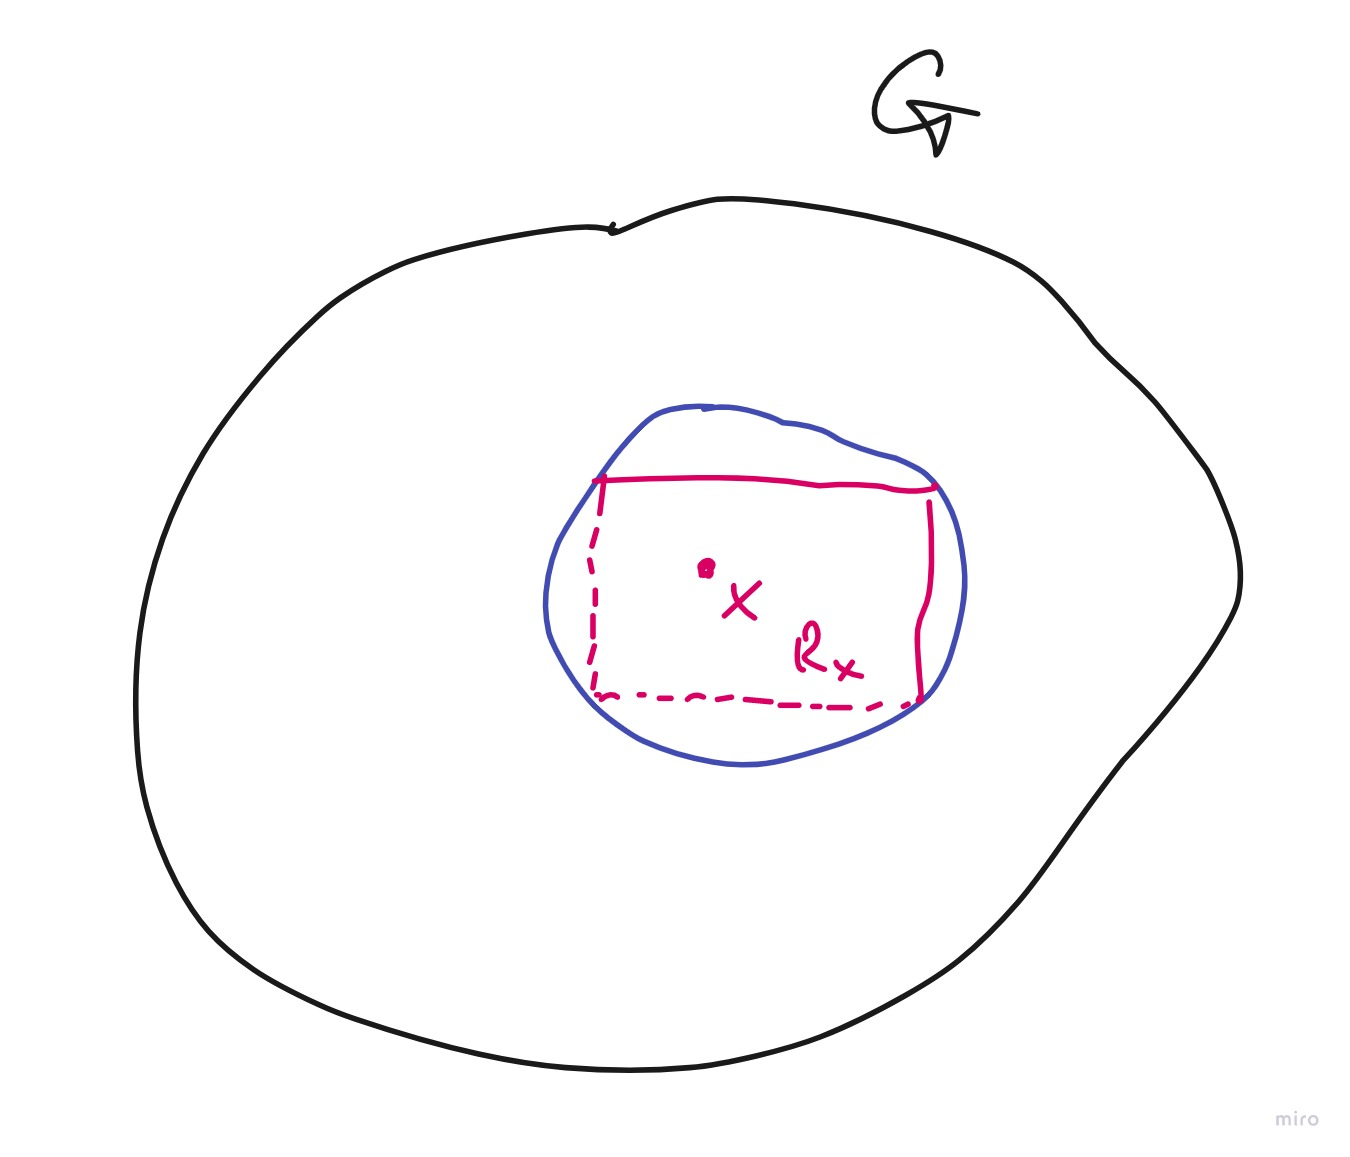
\includegraphics[scale=0.15]{./assets/01-measure-theory/opened-set-with-rect.jpg}
    }

    Выкинем повторы: $G = \bigcup_{n=1}^{\infty} R_{x_n} = \bigsqcup_{n=1}^{\infty} \bigsqcup_{j=1}^{m_n} Q_{nj}$
\end{proof}

\begin{consequence}
    $\mathcal{B}(\mathcal{P}^m_Q) = \mathcal{B}^m$.
\end{consequence}
\begin{proof}
    
    1. $\mathcal{P}^m \supset \mathcal{P}^m_Q \implies \mathcal{B}(\mathcal{P}^m) \supset \mathcal{B}(\mathcal{P}_Q^m)$

    $(a, b] \in \mathcal{B}^m \implies \mathcal{P}^m \subset \mathcal{B}^m \implies \mathcal{B}(\mathcal{P}^m) \subset \mathcal{B}^m$

    $G$ -- открытое $\implies G \in \mathcal{B}(\mathcal{P}_Q^m) \implies \mathcal{B}(\mathcal{P}^m_Q) \supset \mathcal{B}^m$
\end{proof}

\Subsection{Объем и мера}
\begin{definition}
    $\mathcal{P}$ -- полукольцо. $\mu: \mathcal{P} \rightarrow [0, +\infty]$. $\mu$ -- объем, если 

    \begin{enumerate}
        \item $\mu(\emptyset) = 0$
        \item Если $P_1, P_2, \dots, P_n \in \mathcal{P}$ и $\bigsqcup_{k=1}^n P_k \in \mathcal{P}$, то $\mu \left(\bigsqcup_{k=1}^n P_k\right) = \sum_{k=1}^{n} \mu P_k$ 
    \end{enumerate}
\end{definition}

\begin{definition}
    $\mu$ -- мера, если 

    \begin{enumerate}
        \item $\mu(\emptyset) = 0$
        \item Если $P_1, P_2, \dots \in \mathcal{P}$ и $\bigsqcup_{k=1}^{\infty} P_k \in \mathcal{P}$, то $\mu \underbrace{\left(\bigsqcup_{k=1}^{\infty} P_k\right)}_{\text{счетная аддитивность}} = \sum_{k=1}^{\infty} \mu P_k$ 
    \end{enumerate}
\end{definition}

\begin{exerc}
    $\mu$ -- мера. Если $\mu \not \equiv +\infty$, то условия $\mu \emptyset = 0$ выполнено автоматически.
\end{exerc}

\begin{example}
    \begin{enumerate}
        \item $\mathcal{P}^1$,   \;\; $\mu (a, b] := b - a$ -- длина (упр. доказать, что объем и мера).
        \item {
            $g: \mathcal{R} \rightarrow \mathcal{R}$ -- нестрого монотонная

            \begin{enumerate}
                \item $\mu_{g}(a, b] := g(b) - g(a)$ (упр. доказать, что объем).
            \end{enumerate}
        }
        \item $\mathcal{P}^m$ (m-мерные ячейки), \;\; $\mu (a, b] := (b_1 - a_1)(b_2 - a_2) \dots (b_m - a_m), \ a := (a_1, \ ..., \ a_m), \ b := (b_1, \ ..., \ b_m)$ -- классический объем.
        \item {
            $\mathcal{P} = 2^X$, \;\; $x_0 \in X$, \;\; $a \geq 0$
            
            \begin{equation}
                \mu A := 
                \begin{cases}
                    $a$, \ if \  x_{0} \in A \\
                    $0$, \ otherwise
                \end{cases}                
            \end{equation}

            $\mu$ - мера.
        }
        \item {
            $\mathcal{P}$ -- огр. мн-ва и их дополнения.
            
            \begin{equation}
                \mu A := 
                \begin{cases}
                    $1$, \ if \  x_{0} \in A \\
                    $0$, \ otherwise
                \end{cases}                
            \end{equation}

            $\mu$ - объем, но не мера.
        }
    \end{enumerate}
\end{example}

\begin{theorem}
    $\mu$ - объем на полукольце $\mathcal{P}$

    \begin{enumerate}
        \item Монотонность: $\mathcal{P} \ni P \subset \tilde{P} \in \mathcal{P} \implies \mu P \leq \mu \tilde{P}$
        \item {
            \begin{enumerate}
                \item Усиленная монотонность: $P_1, P_2, \dots P_n, P \in \mathcal{P}$. $\bigsqcup_{k=1}^n P_k \subset P \implies \sum_{k=1}^n \mu P_k \leq \mu P$
                \item Пункт (a), но $n = \infty$
            \end{enumerate}
        }
        \item Полуаддитивность: $P, P_1, P_2, \dots P_n \in \mathcal{P}$ и $P \subset \bigcup_{k=1}^{n}P_k$, тогда $\mu P \leq \sum_{k=1}^{n} \mu P_k$ 
    \end{enumerate}
\end{theorem}

\begin{proof}
    \begin{enumerate}
        \item Очев типо.
        \item {
        \begin{enumerate}
            \item $P \setminus \bigsqcup_{k=1}^{n} \mu P_k =  \bigsqcup_{j=1}^{m} Q_j \implies P = \bigsqcup_{k=1}^{n} P_k \sqcup \bigsqcup_{j=1}^m Q_j \implies \mu P = \sum_{k=1}^{n} \mu P_k + \sum_{j=1}^{m} \mu Q_j \geq \sum_{k=1}^{n} \mu P_k $
            \item $\bigsqcup_{k=1}^{\infty} P_k \subset P \implies \bigsqcup_{k=1}^n P_k \subset P \implies \sum_{k=1}^{n} \mu P_k \rightarrow \sum_{k=1}^{\infty} \mu P_k \leq \mu P$
        \end{enumerate}
        \item {
            $P_k' := P \cap P_k \in \mathcal{P}$ ($\mathcal{P}$ - полукольцо), \;\; $P = \bigcup_{k=1}^{n} P_k' = \bigsqcup_{k=1}^{n} \underbrace{\bigsqcup_{j=1}^{m_k} Q_{kj}}_{\in P_k'} \implies$
            
            $\implies \mu P = \sum_{k=1}^n \underbrace{\sum_{j=1}^{m_k} \mu Q_{kj}}_{\leq \mu P'_k \leq \mu P_k \ (property \ 2(a). )} \leq \sum_{k=1}^n \mu P_k$
        }
        }
    \end{enumerate}
\end{proof}

\begin{remark}
    \begin{enumerate}
        \item {
            Если $\mathcal{P}$ -- кольцо и $A, B$ ($B \subset A$) $ \in \mathcal{P}$, то $A \setminus B \in \mathcal{P}$

            $\mu (A \setminus B) + \mu B = \mu A$

            Если $\mu B \neq +\infty$, то $\mu (A \setminus B) = \mu A - \mu B$
        }
    \end{enumerate}
\end{remark}

\begin{theorem}
    $\mathcal{P}$ -- полукольцо подмн-в $X$, \mu -- объем на $\mathcal{P}$

    $\mathcal{Q}$ -- полукольцо подмн-в $Y$, \nu -- объем на $\mathcal{Q}$

    $\lambda(P \times Q) := \mu P \cdot \nu Q$, где $0 \cdot +\infty = +\infty \cdot 0 = 0$

    Тогда $\lambda$ -- объем на $P \times Q$.
\end{theorem}
\begin{consequence}
    Классический объем на ячейках -- действительно объем.
\end{consequence}
\begin{proof}
    Простой случай. $P = \bigsqcup_{k=1}^{n}P_k, Q = \bigsqcup_{j=1}^m Q_j$, тогда:

    $P \times Q = \bigsqcup_{k=1}^{n} \bigsqcup_{j=1}^{m} P_k \times Q_j$, докажем, что $\underbrace{\lambda (P \times Q)}_{\sum_{k=1}^n \mu P_k \cdot \sum_{j=1}^m \nu Q_j = \mu P \cdot \nu Q} = \sum_{k=1}^n \sum_{j=1}^m \underbrace{\lambda (P_k \times Q_j)}_{\mu P_k \cdot \nu Q_j}$

    Общий случай.

    \begin{center}
        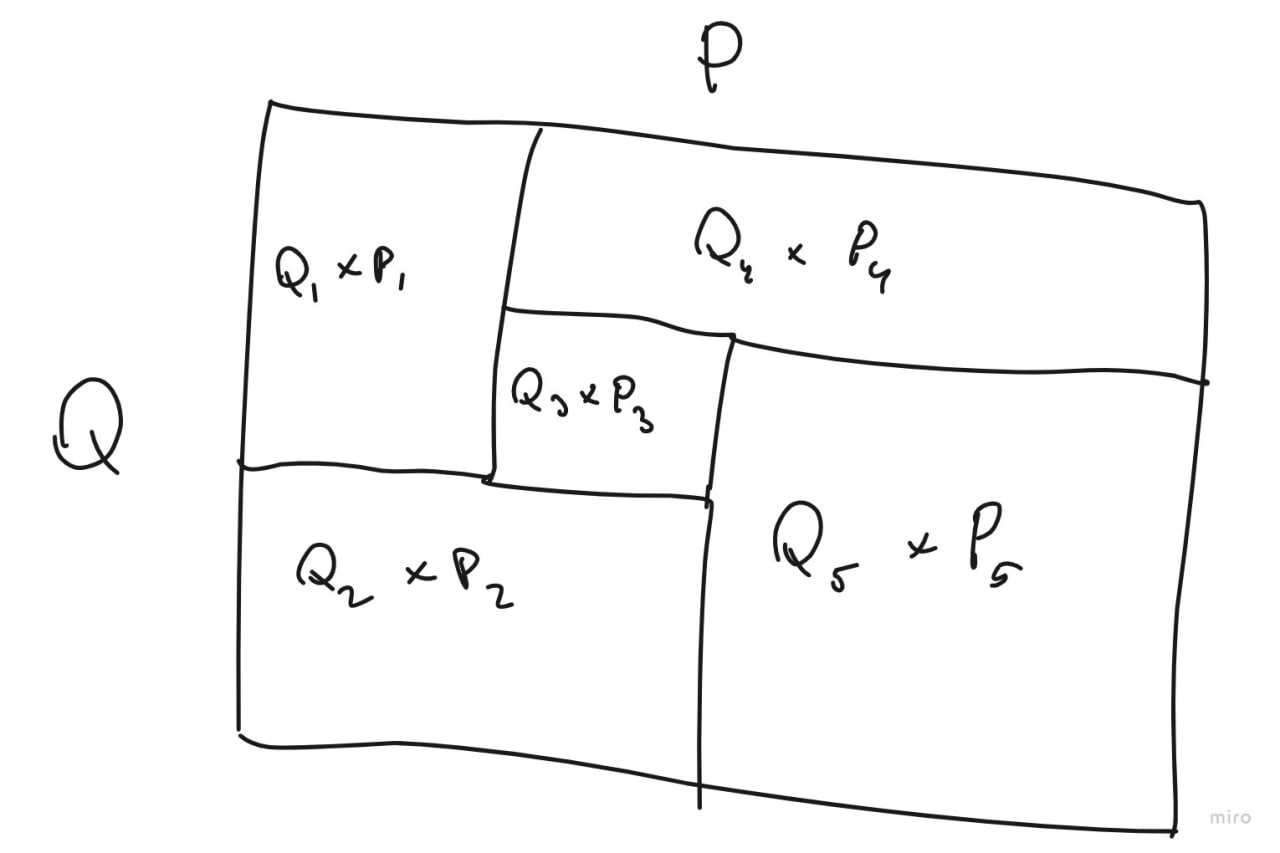
\includegraphics[scale=0.3]{./assets/01-measure-theory/PxQ.jpg}
    \end{center}

    $P \times Q = \bigsqcup_{k=1}^{n} P_k \times Q_k$
    
    $P = \bigcup_{k=1}^{n} P_k = \bigsqcup_{k=1}^{N} P_k'$

    $Q = \bigcup_{j=1}^{m} Q_j = \bigsqcup_{j=1}^{M} Q_j'$
\end{proof}

\begin{example}
    \begin{enumerate}
        \item Классический объем на ячейках $\lambda_m$ -- мера
        \item {
            $g : \mathbb{R} \rightarrow \mathbb{R}$ нестрого монотонная возрастающая и непрерывна слева во всех точках, тогда $\nu_g (a, b]:=g(b) - g(a)$ -- мера.

            (\underline{Rem}: $lim_{x \rightarrow a-} f(x) = f(a)$ -- непрерывность слева).
        }
        \item Считающаяся мера: $\mu A := \#A$ -- кол-во элементов.
        \item $T = \{t_1, t_2, \dots \}$ -- не более чем счетное множетсво, $w_1, w_2, \dots \geq 0$, $\mu A := \sum_{k: t_k \in A} w_k$ $\rightarrow$ $\mu$ -- мера.
    \end{enumerate}
\end{example}

\begin{proof}
    4. $A = \bigsqcup_{n=1}^{\infty} A_n \implies \mu A = \sum_{n=1}^{\infty} \mu A_n$

    Обозначения:

    \begin{enumerate}
        \item $\sum_{n=1}^{N} \sum_{k: \ t_k \in A_n} w_k \ (*)$.
        \item $\sum_{k: \ t_k \in A} w_k \ (**)$.
        \item $\sum_{n=1}^{\infty} \sum_{k: \ t_k \in A_n} w_k \ (***)$.
    \end{enumerate}

    \begin{enumerate}
        \item {
            $\mu A = \sum_{k: \ t_k \in A} w_k \ (**) \geq \sum_{n=1}^{N} \sum_{k: \ t_k \in A_n} w_k \ (*)$ -- т.к. $A_i \cap A_j = \emptyset \ (\forall i, \ j: \ i \neq j)$, то каждое слагаемое $w_k$ не более $1$ раза попадет в $(*)$ и $A = \bigsqcup_{n=1}^{\infty} A_n$.
        }

        \item {
            $\sum_{n=1}^{\infty} \mu A_n = \sum_{n=1}^{\infty} \sum_{k: \ t_k \in A_n} w_k \ (***) \geq \sum_{k: \ t_k \in A}$ -- нер-во верно, так как мы можем к каждому $w_k$ из $(**)$ найти этот же $w_k$ в $(***)$. 
        }

        Итого имеем равенство:

        $(**) = (***): \ \sum_{k: \ t_k \in A} w_k = \sum_{n=1}^{\infty} \sum_{k: \ t_k \in A_n} w_k \implies \mu A = \sum_{n=1}^{\infty} \mu A_n$, чтд.

        (\underline{От автора}: если у кого-то лучше расписано данное док-во, сделайте, пожалуйста, PR).
    \end{enumerate}

\end{proof}
